\documentclass{standalone}
\usepackage{tikz, xcolor}
\usetikzlibrary{graphs,quotes,positioning}


% custom SUNY Poly color scheme
\definecolor{poly-gold}{rgb}{0.91,0.624,0.114}
\definecolor{poly-blue}{rgb}{0.122,0.184,0.392}
% colored text commands
\newcommand{\pgold}[1]{{\color{poly-gold} #1}}
\newcommand{\pblue}[1]{{\color{poly-blue} #1}}

\begin{document}

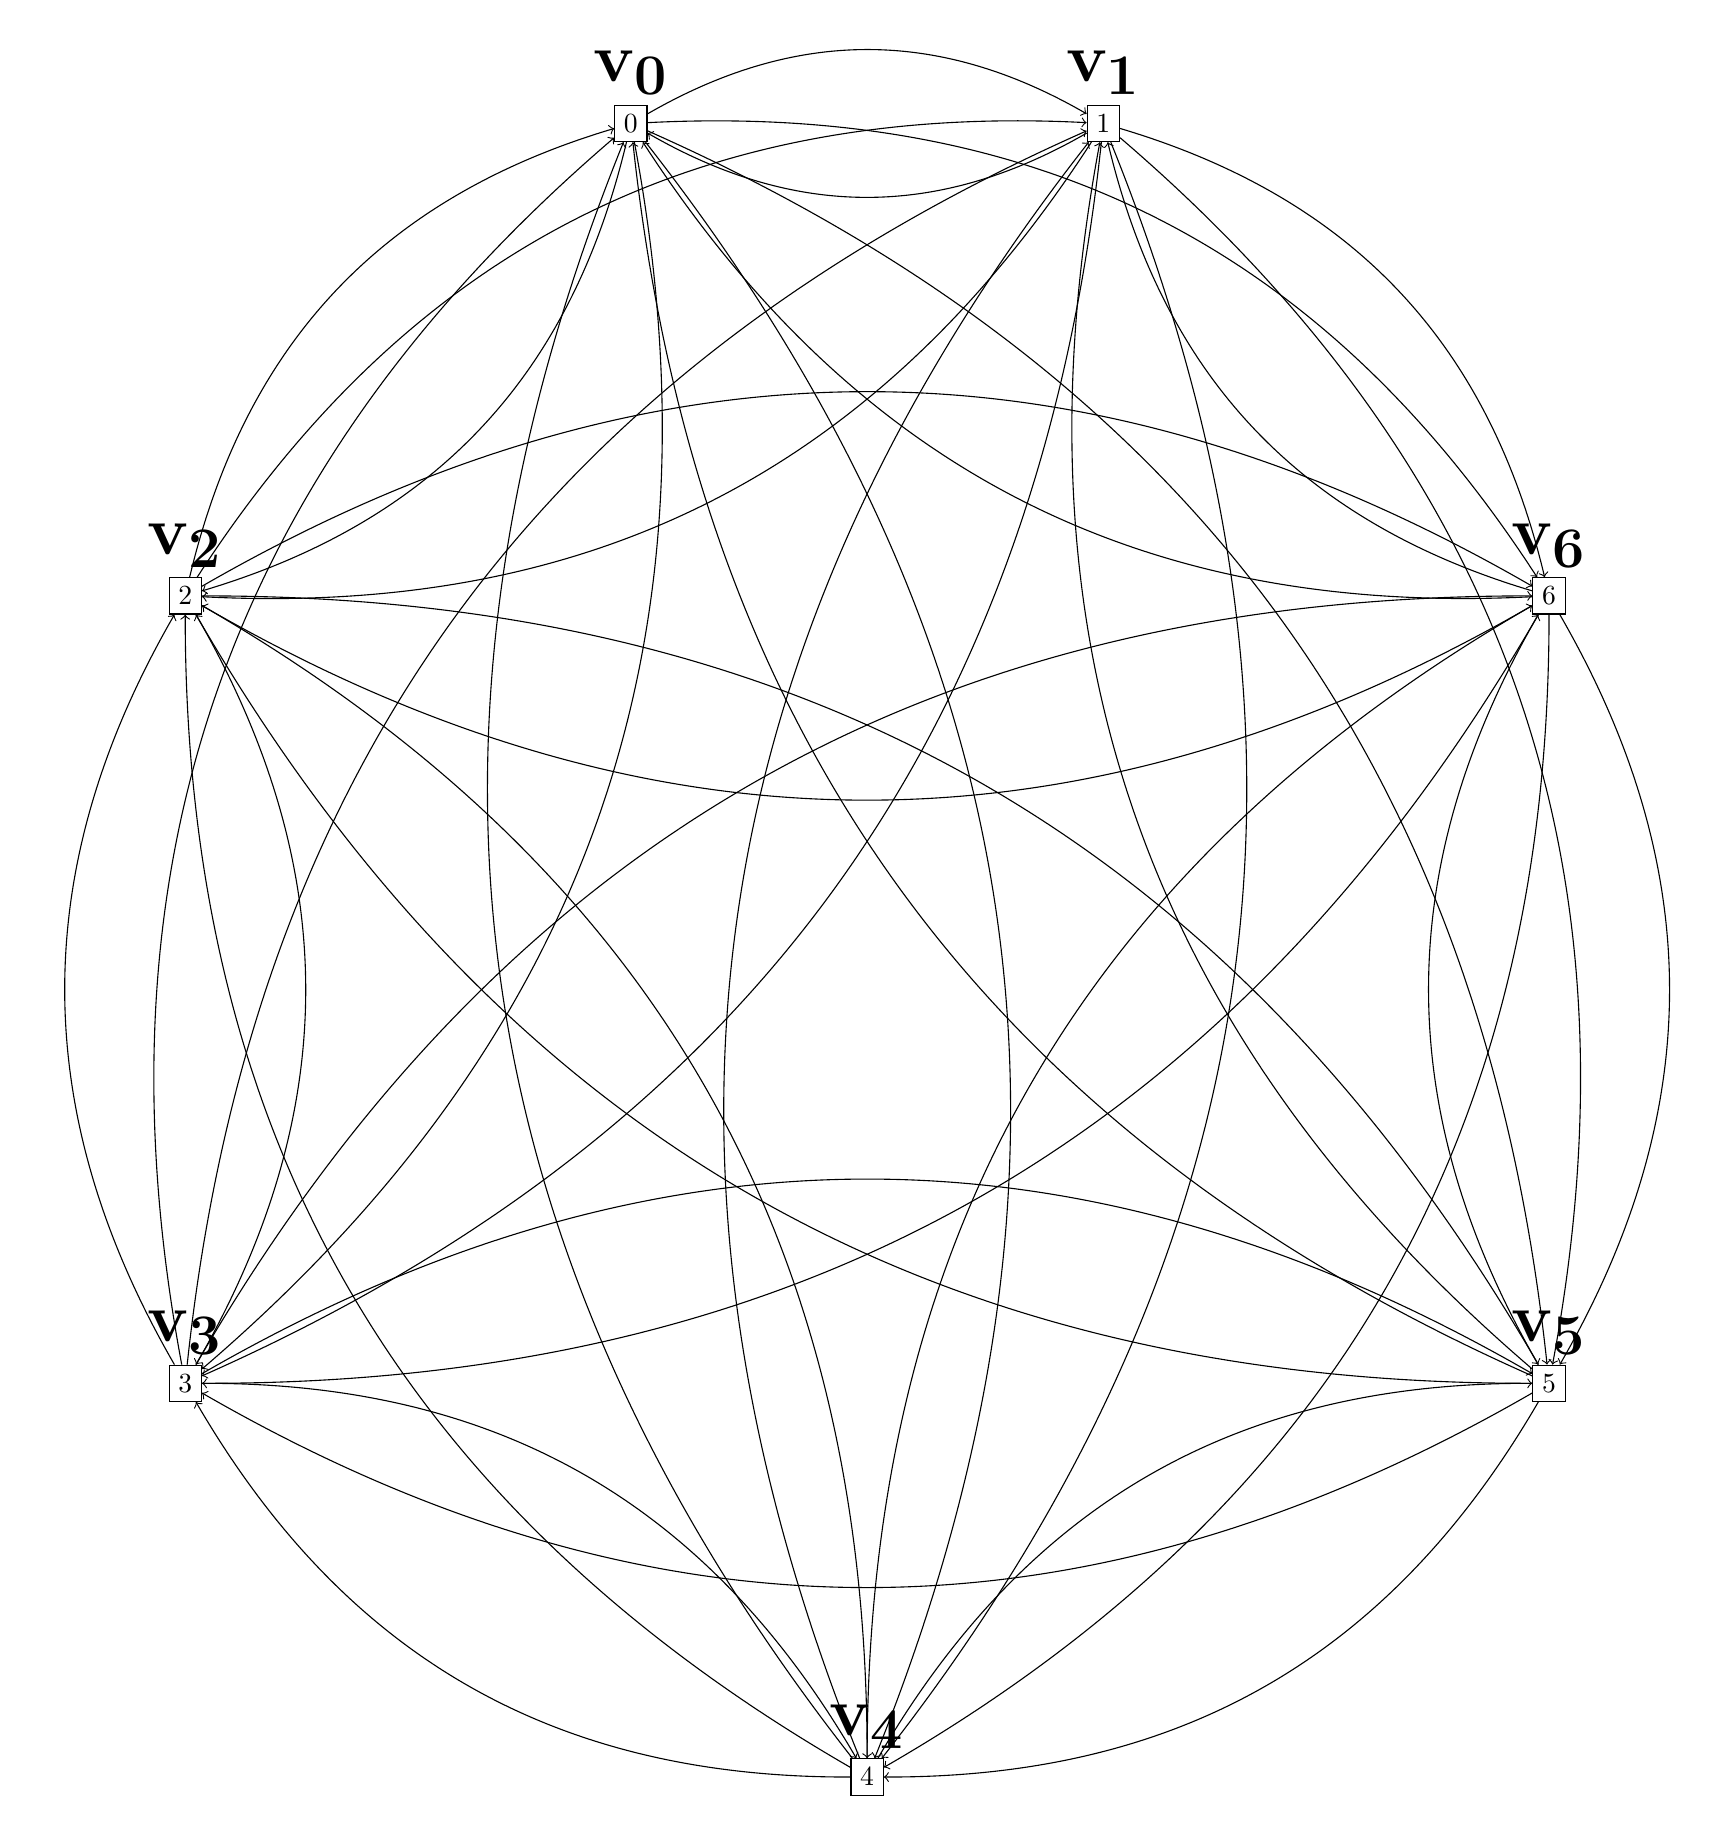
\begin{tikzpicture}
    \graph [nodes = {rectangle, draw},
                    circular placement,
                    radius = 10cm] {
                        0[xshift=-3cm, yshift=1cm, label=\Huge $\mathbf{v_0}$] ->[bend left] 1[xshift=3cm, label=\Huge $\mathbf{v_1}$],
                        0 ->[bend left] 2[label=\Huge $\mathbf{v_2}$],
                        0 ->[bend left] 3[label=\Huge $\mathbf{v_3}$],
                        0 ->[bend left] 4[label=\Huge $\mathbf{v_4}$],
                        0 ->[bend left] 5[label=\Huge $\mathbf{v_5}$],
                        0 ->[bend left] 6[label=\Huge $\mathbf{v_6}$],
                        1 ->[bend left] 0,
                        1 ->[bend left] 2,
                        1 ->[bend left] 3,
                        1 ->[bend left] 4,
                        1 ->[bend left] 5,
                        1 ->[bend left] 6,
                        2 ->[bend left] 0,
                        2 ->[bend left] 1,
                        2 ->[bend left] 3,
                        2 ->[bend left] 4,
                        2 ->[bend left] 5,
                        2 ->[bend left] 6,
                        3 ->[bend left] 0,
                        3 ->[bend left] 2,
                        3 ->[bend left] 1,
                        3 ->[bend left] 4,
                        3 ->[bend left] 5,
                        3 ->[bend left] 6,
                        4 ->[bend left] 0,
                        4 ->[bend left] 1,
                        4 ->[bend left] 3,
                        4 ->[bend left] 2,
                        4 ->[bend left] 5,
                        4 ->[bend left] 6,
                        5 ->[bend left] 0,
                        5 ->[bend left] 2,
                        5 ->[bend left] 1,
                        5 ->[bend left] 4,
                        5 ->[bend left] 3,
                        5 ->[bend left] 6,
                        6 ->[bend left] 0,
                        6 ->[bend left] 1,
                        6 ->[bend left] 3,
                        6 ->[bend left] 2,
                        6 ->[bend left] 5,
                        6 ->[bend left] 4,
                        };
\end{tikzpicture}
\end{document}